\documentclass[tikz,border=10pt]{standalone}
\usepackage{tikz}
\usetikzlibrary{shapes.geometric,arrows.meta,positioning,fit,backgrounds,shadows,decorations.pathreplacing,shapes.multipart,shapes.symbols}

\begin{document}
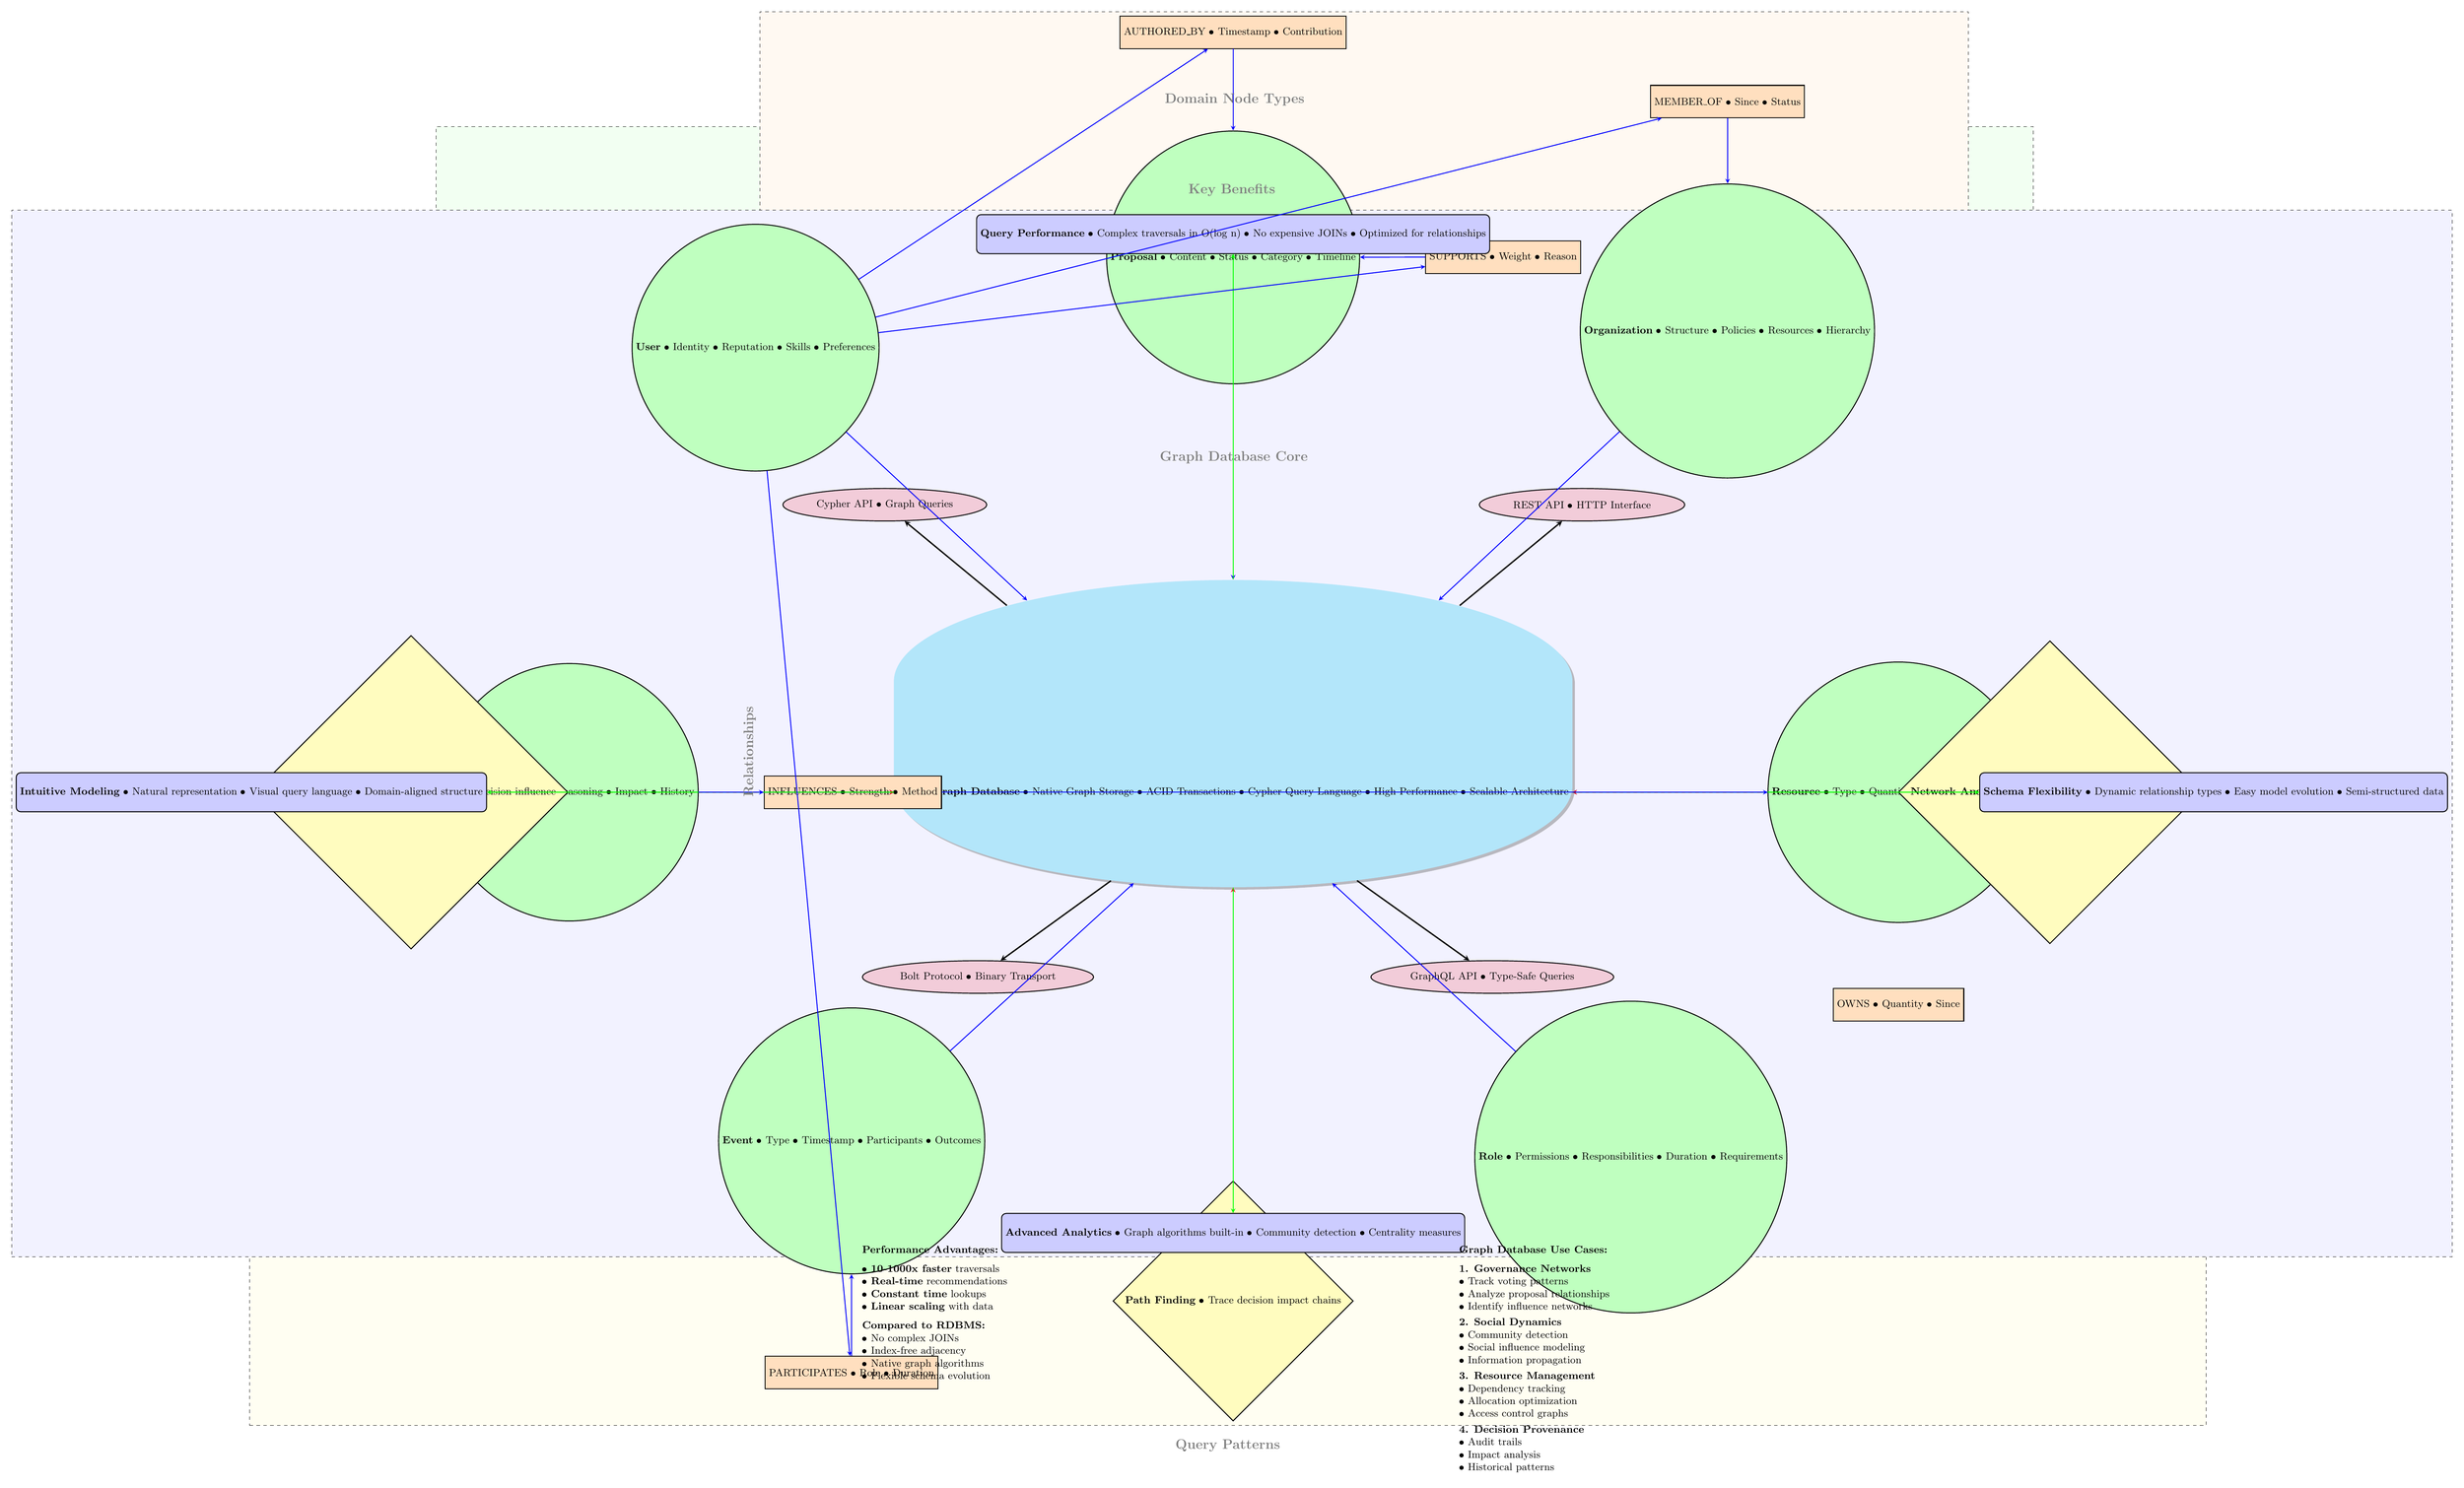
\begin{tikzpicture}[scale=2.5,
    node distance=6cm,
    every node/.style={font=\small},
    % Graph Database Components
    graphdb/.style={cylinder,shape border rotate=90,aspect=0.3,minimum height=2cm,minimum width=2.8cm,fill=cyan!30,thick,drop shadow},
    node_type/.style={circle,draw,minimum size=1.5cm,fill=green!25,thick},
    relationship/.style={rectangle,draw,minimum width=2.2cm,minimum height=1cm,fill=orange!25,thick},
    query/.style={diamond,draw,minimum width=2cm,minimum height=1.4cm,fill=yellow!25,thick},
    benefit/.style={rectangle,draw,minimum width=2.5cm,minimum height=1.2cm,fill=blue!20,thick,rounded corners},
    api/.style={ellipse,draw,minimum width=2.2cm,minimum height=1cm,fill=purple!20,thick},
    arrow/.style={->,>=stealth,very thick},
    data_flow/.style={->,>=stealth,thick,blue},
    query_flow/.style={->,>=stealth,thick,red,dashed},
    benefit_arrow/.style={->,>=stealth,thick,green}
]

% Central Graph Database
\node[graphdb] (neo4j) {
    \textbf{Neo4j Graph Database} • Native Graph Storage • ACID Transactions • Cypher Query Language • High Performance • Scalable Architecture
};

% Node Types in Virtual Utopia
\node[node_type,above left=5cm and 6cm of neo4j] (user_node) {
    \textbf{User} • Identity • Reputation • Skills • Preferences
};

\node[node_type,above=6cm of neo4j] (proposal_node) {
    \textbf{Proposal} • Content • Status • Category • Timeline
};

\node[node_type,above right=5cm and 6cm of neo4j] (org_node) {
    \textbf{Organization} • Structure • Policies • Resources • Hierarchy
};

\node[node_type,left=6cm of neo4j] (decision_node) {
    \textbf{Decision} • Outcome • Reasoning • Impact • History
};

\node[node_type,right=6cm of neo4j] (resource_node) {
    \textbf{Resource} • Type • Quantity • Location • Ownership
};

\node[node_type,below left=5cm and 6cm of neo4j] (event_node) {
    \textbf{Event} • Type • Timestamp • Participants • Outcomes
};

\node[node_type,below right=5cm and 6cm of neo4j] (role_node) {
    \textbf{Role} • Permissions • Responsibilities • Duration • Requirements
};

% Relationship Types
\node[relationship,above=2.5cm of proposal_node] (authored_by) {AUTHORED\_BY • Timestamp • Contribution};
\node[relationship,right=2cm of proposal_node] (supports) {SUPPORTS • Weight • Reason};
\node[relationship,above=2cm of org_node] (member_of) {MEMBER\_OF • Since • Status};
\node[relationship,right=2cm of decision_node] (influences) {INFLUENCES • Strength • Method};
\node[relationship,below=2cm of resource_node] (owns) {OWNS • Quantity • Since};
\node[relationship,below=2.5cm of event_node] (participates) {PARTICIPATES • Role • Duration};

% Query Examples
\node[query,left=10cm of neo4j] (influence_query) {
    \textbf{Influence Analysis} • Find users with high decision influence
};

\node[query,right=10cm of neo4j] (network_query) {
    \textbf{Network Analysis} • Detect community clusters \& bridges
};

\node[query,below=9cm of neo4j] (path_query) {
    \textbf{Path Finding} • Trace decision impact chains
};

% Benefits
\node[benefit,above=10cm of neo4j] (performance_benefit) {
    \textbf{Query Performance} • Complex traversals in O(log n) • No expensive JOINs • Optimized for relationships
};

\node[benefit,right=12.5cm of neo4j] (flexibility_benefit) {
    \textbf{Schema Flexibility} • Dynamic relationship types • Easy model evolution • Semi-structured data
};

\node[benefit,below=10cm of neo4j] (analytics_benefit) {
    \textbf{Advanced Analytics} • Graph algorithms built-in • Community detection • Centrality measures
};

\node[benefit,left=12.5cm of neo4j] (intuitive_benefit) {
    \textbf{Intuitive Modeling} • Natural representation • Visual query language • Domain-aligned structure
};

% APIs and Integration
\node[api,above left=2.5cm and 2.5cm of neo4j] (cypher_api) {Cypher API • Graph Queries};
\node[api,above right=2.5cm and 2.5cm of neo4j] (rest_api) {REST API • HTTP Interface};
\node[api,below left=2.5cm and 2.5cm of neo4j] (bolt_api) {Bolt Protocol • Binary Transport};
\node[api,below right=2.5cm and 2.5cm of neo4j] (graphql_api) {GraphQL API • Type-Safe Queries};

% Background groupings
\begin{scope}[on background layer]
\node[fill=cyan!5,draw,dashed,fit=(neo4j)(cypher_api)(rest_api)(bolt_api)(graphql_api)] (db_group) {};
\node[fill=green!5,draw,dashed,fit=(user_node)(proposal_node)(org_node)(decision_node)(resource_node)(event_node)(role_node)] (nodes_group) {};
\node[fill=orange!5,draw,dashed,fit=(authored_by)(supports)(member_of)(influences)(owns)(participates)] (relationships_group) {};
\node[fill=yellow!5,draw,dashed,fit=(influence_query)(network_query)(path_query)] (queries_group) {};
\node[fill=blue!5,draw,dashed,fit=(performance_benefit)(flexibility_benefit)(analytics_benefit)(intuitive_benefit)] (benefits_group) {};
\end{scope}

% Data Flow Connections
\draw[data_flow] (user_node) -- (neo4j);
\draw[data_flow] (proposal_node) -- (neo4j);
\draw[data_flow] (org_node) -- (neo4j);
\draw[data_flow] (decision_node) -- (neo4j);
\draw[data_flow] (resource_node) -- (neo4j);
\draw[data_flow] (event_node) -- (neo4j);
\draw[data_flow] (role_node) -- (neo4j);

% API Connections
\draw[arrow] (neo4j) -- (cypher_api);
\draw[arrow] (neo4j) -- (rest_api);
\draw[arrow] (neo4j) -- (bolt_api);
\draw[arrow] (neo4j) -- (graphql_api);

% Query Connections
\draw[query_flow] (influence_query) -- (neo4j);
\draw[query_flow] (network_query) -- (neo4j);
\draw[query_flow] (path_query) -- (neo4j);

% Benefit Connections
\draw[benefit_arrow] (neo4j) -- (performance_benefit);
\draw[benefit_arrow] (neo4j) -- (flexibility_benefit);
\draw[benefit_arrow] (neo4j) -- (analytics_benefit);
\draw[benefit_arrow] (neo4j) -- (intuitive_benefit);

% Relationship Connections (showing examples)
\draw[data_flow] (user_node) -- (authored_by);
\draw[data_flow] (authored_by) -- (proposal_node);
\draw[data_flow] (user_node) -- (supports);
\draw[data_flow] (supports) -- (proposal_node);
\draw[data_flow] (user_node) -- (member_of);
\draw[data_flow] (member_of) -- (org_node);

% Cross-domain relationships
\draw[data_flow] (decision_node) -- (influences);
\draw[data_flow] (influences) -- (resource_node);
\draw[data_flow] (user_node) -- (participates);
\draw[data_flow] (participates) -- (event_node);

% Labels
\node[above=0.5cm of db_group,font=\large,text=gray] {\textbf{Graph Database Core}};
\node[above=0.5cm of nodes_group,font=\large,text=gray] {\textbf{Domain Node Types}};
\node[left=0.3cm of relationships_group,font=\large,text=gray,rotate=90] {\textbf{Relationships}};
\node[below=0.3cm of queries_group,font=\large,text=gray] {\textbf{Query Patterns}};
\node[above=0.3cm of benefits_group,font=\large,text=gray] {\textbf{Key Benefits}};

% Use Case Examples
\node[below right=11cm and 4cm of neo4j,font=\small,align=left] (use_cases) {
    \textbf{Graph Database Use Cases:}\\[0.2cm]
    \textbf{1. Governance Networks}\\
    • Track voting patterns\\
    • Analyze proposal relationships\\
    • Identify influence networks\\[0.1cm]
    \textbf{2. Social Dynamics}\\
    • Community detection\\
    • Social influence modeling\\
    • Information propagation\\[0.1cm]
    \textbf{3. Resource Management}\\
    • Dependency tracking\\
    • Allocation optimization\\
    • Access control graphs\\[0.1cm]
    \textbf{4. Decision Provenance}\\
    • Audit trails\\
    • Impact analysis\\
    • Historical patterns
};

% Performance Metrics
\node[below left=11cm and 4cm of neo4j,font=\small,align=left] (metrics) {
    \textbf{Performance Advantages:}\\[0.2cm]
    • \textbf{10-1000x faster} traversals\\
    • \textbf{Real-time} recommendations\\
    • \textbf{Constant time} lookups\\
    • \textbf{Linear scaling} with data\\[0.2cm]
    \textbf{Compared to RDBMS:}\\
    • No complex JOINs\\
    • Index-free adjacency\\
    • Native graph algorithms\\
    • Flexible schema evolution
};

\end{tikzpicture}
\end{document}
